%Latex->PDF
%
% TRUCJE (afhankelijk van de bestandsnaam, krijg je de handout of de presentatie ...
% (!! GEBRUIK LINUX HARD LINKS OM HETZELFDE BESTAND TWEE NAMEN TE GEVEN !!)
% See https://tex.stackexchange.com/questions/197330/how-can-i-check-if-the-filename-of-a-latex-document-contains-a-string
%
\RequirePackage{substr}   % RequirePackage omdat \usepackage niet werkt voor \begin{document} !

\begingroup\escapechar=-1
\xdef\handoutstring{\string\handout}   % dirty hack, omdat anders stringcompare niet werkt
\endgroup

\IfSubStringInString{\handoutstring}{\jobname}
{
\documentclass[aspectratio=169,handout]{beamer}
\wlog{We genereren de HANDOUT versie voor \jobname.}
}{
\documentclass[aspectratio=169]{beamer}
\wlog{We genereren de PRESENTATIE versie voor \jobname.}
}
% EndofTrucje


\usepackage[dutch]{babel}
\usepackage{amssymb,amsmath,amsthm}

\usepackage{cancel}
\usepackage{relsize}

\usepackage{listings}
\usepackage{xcolor}
%\usepackage{verbatim}

\usepackage{qrcode}

\setbeamertemplate{headline}{\insertframenumber/\inserttotalframenumber}
\newcommand{\ds}{\displaystyle}
\newcommand{\N}{\ensuremath{\mathbb{N}}}
\newcommand{\Z}{\ensuremath{\mathbb{Z}}}
\newcommand{\Nnul}{\ensuremath{\mathbb{N}_0}}
\newcommand{\Q}{\ensuremath{\mathbb{Q}}}
\newcommand{\R}{\ensuremath{\mathbb{R}}}
\newcommand{\perdef}{\overset{\mathrm{def}}{=}}
\newcommand{\Bgsin}{\mathrm{Bgsin}\,}
\newcommand{\Bgcos}{\mathrm{Bgcos}\,}
\newcommand{\Bgtan}{\mathrm{Bgtan}\,}

\DeclareMathOperator{\dom}{dom}     % domein
\DeclareMathOperator{\codom}{codom} % codomein
\DeclareMathOperator{\bld}{bld}     % beeld
\DeclareMathOperator{\graf}{graf}   % grafiek
\DeclareMathOperator{\rico}{rico}   % richtingcoëfficient
\DeclareMathOperator{\co}{co}       % coordinaat

\newtheorem*{eigenschap}{Eigenschap}

\newcommand{\p}{\pause}
\newcommand{\important}[1]{\ensuremath{\colorbox{lightgray}{$#1$}}}

\providecommand{\blue}[1]{{\color{blue}#1}}  
\providecommand{\red}[1]{{\color{red}#1}}  

\usepackage{pgf,tikz,pgfplots}
%\pgfplotsset{compat=1.15}
\usepackage{mathrsfs}
\usepackage{dsfont}
\usepackage{relsize}   % voor \mathlarger
\usetikzlibrary{arrows}
 \usepgfplotslibrary{fillbetween}
 \usetikzlibrary{positioning, fit, calc} 
 \usetikzlibrary{intersections}
 \usetikzlibrary{shapes}
%\pagestyle{empty}



\usepackage{rawfonts}
%\input{prepictex}
%\input{pictex}
%\input{postpictex}

\graphicspath{
	{../../}
	{../}
	{./}
  	{../../pictures/}
   	{../pictures/}
   	{./pictures/}
}

\title{Ximera @ TUG2024}
% \date{\qrcode{https://github.com/XimeraProject}}
\author{Wim Obbels, and Bart Snapp and Jim Fowler}
\date{July 19 2024}
\usetheme{CambridgeUS}
\usecolortheme{seahorse}

\begin{document}

\tikzset{block/.style={draw, thick, text width=3cm , minimum height=2cm, % align=center,
     rectangle split, 
     rectangle split ignore empty parts, 
     rectangle split parts=3,
     rectangle split part align={center, left},
     rounded corners=0.2cm,
     draw},   
     line/.style={-latex}     
}  

\begin{frame}
  \titlepage
\end{frame}

\begin{frame}[t]{\Large\blue{Ximera}}
  \p
  \begin{itemize}[<+->]
  % \item is pronounced \lq chimera\rq 
  \item stands for \hfill \qrcode{https://github.com/XimeraProject}
      \\[-0.5cm]
     {\Large\blue X}imera: {\Large\blue I}nteractive {\Large\blue M}athematical {\Large\blue E}ducational {\Large\blue R}esources for {\Large\blue A}ll
     \\[0.4cm]
  \item is an \textbf{open-source platform}, found on \url{https://github.com/XimeraProject}
  \item supports authoring and publishing \textbf{{\color{blue}interactive} educational content}
  \item such as worksheets, assessments, textbooks and online courses. 
  \item both in \textbf{HTML} (online) and as \textbf{PDF} (online or printed)
  \item authors only write \LaTeX %, most \LaTeX constructs are supported
  \end{itemize}
   
  \vfill

  \p The ultimate goal: promote sustained student success and savings.
  
  % The Ximera Project is funded 2024-2026 with (no other external funding) by a $2,125,000 Open Textbooks Pilot Program grant. In the past, the Ximera Project has also recieved support from NSF Grant DUE-1245433, the Shuttleworth Foundation, the Ohio State University Department of Mathematics, and the Affordable Learning Exchange at OSU. 
  

\end{frame}


\begin{frame}[t]{What does Ximera do ?}
  
%  \providecommand{\answer}[1]{\blue{#1}}
% \begin{enumerate}
%     \item $\mu$     (presumed population mean)      = $\answer{400}$
%     \item $\sigma$  (population standard deviation) = $\answer{25}$
%     \item $\bar{x}$ (sample mean)                   = $\answer{410}$
%     \item $n$       (sample size)                   = $\answer{100}$
% \end{enumerate}
%   \begin{lstlisting}
%     hallo 
% \end{lstlisting}

\begin{center}
  \resizebox{0.5\linewidth}{!}{
    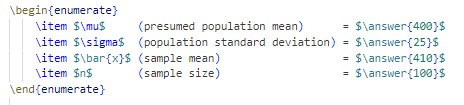
\includegraphics{SimultaneousOutputSource.jpg}
  }  
  \vfill
  \resizebox{0.6\linewidth}{!}{
    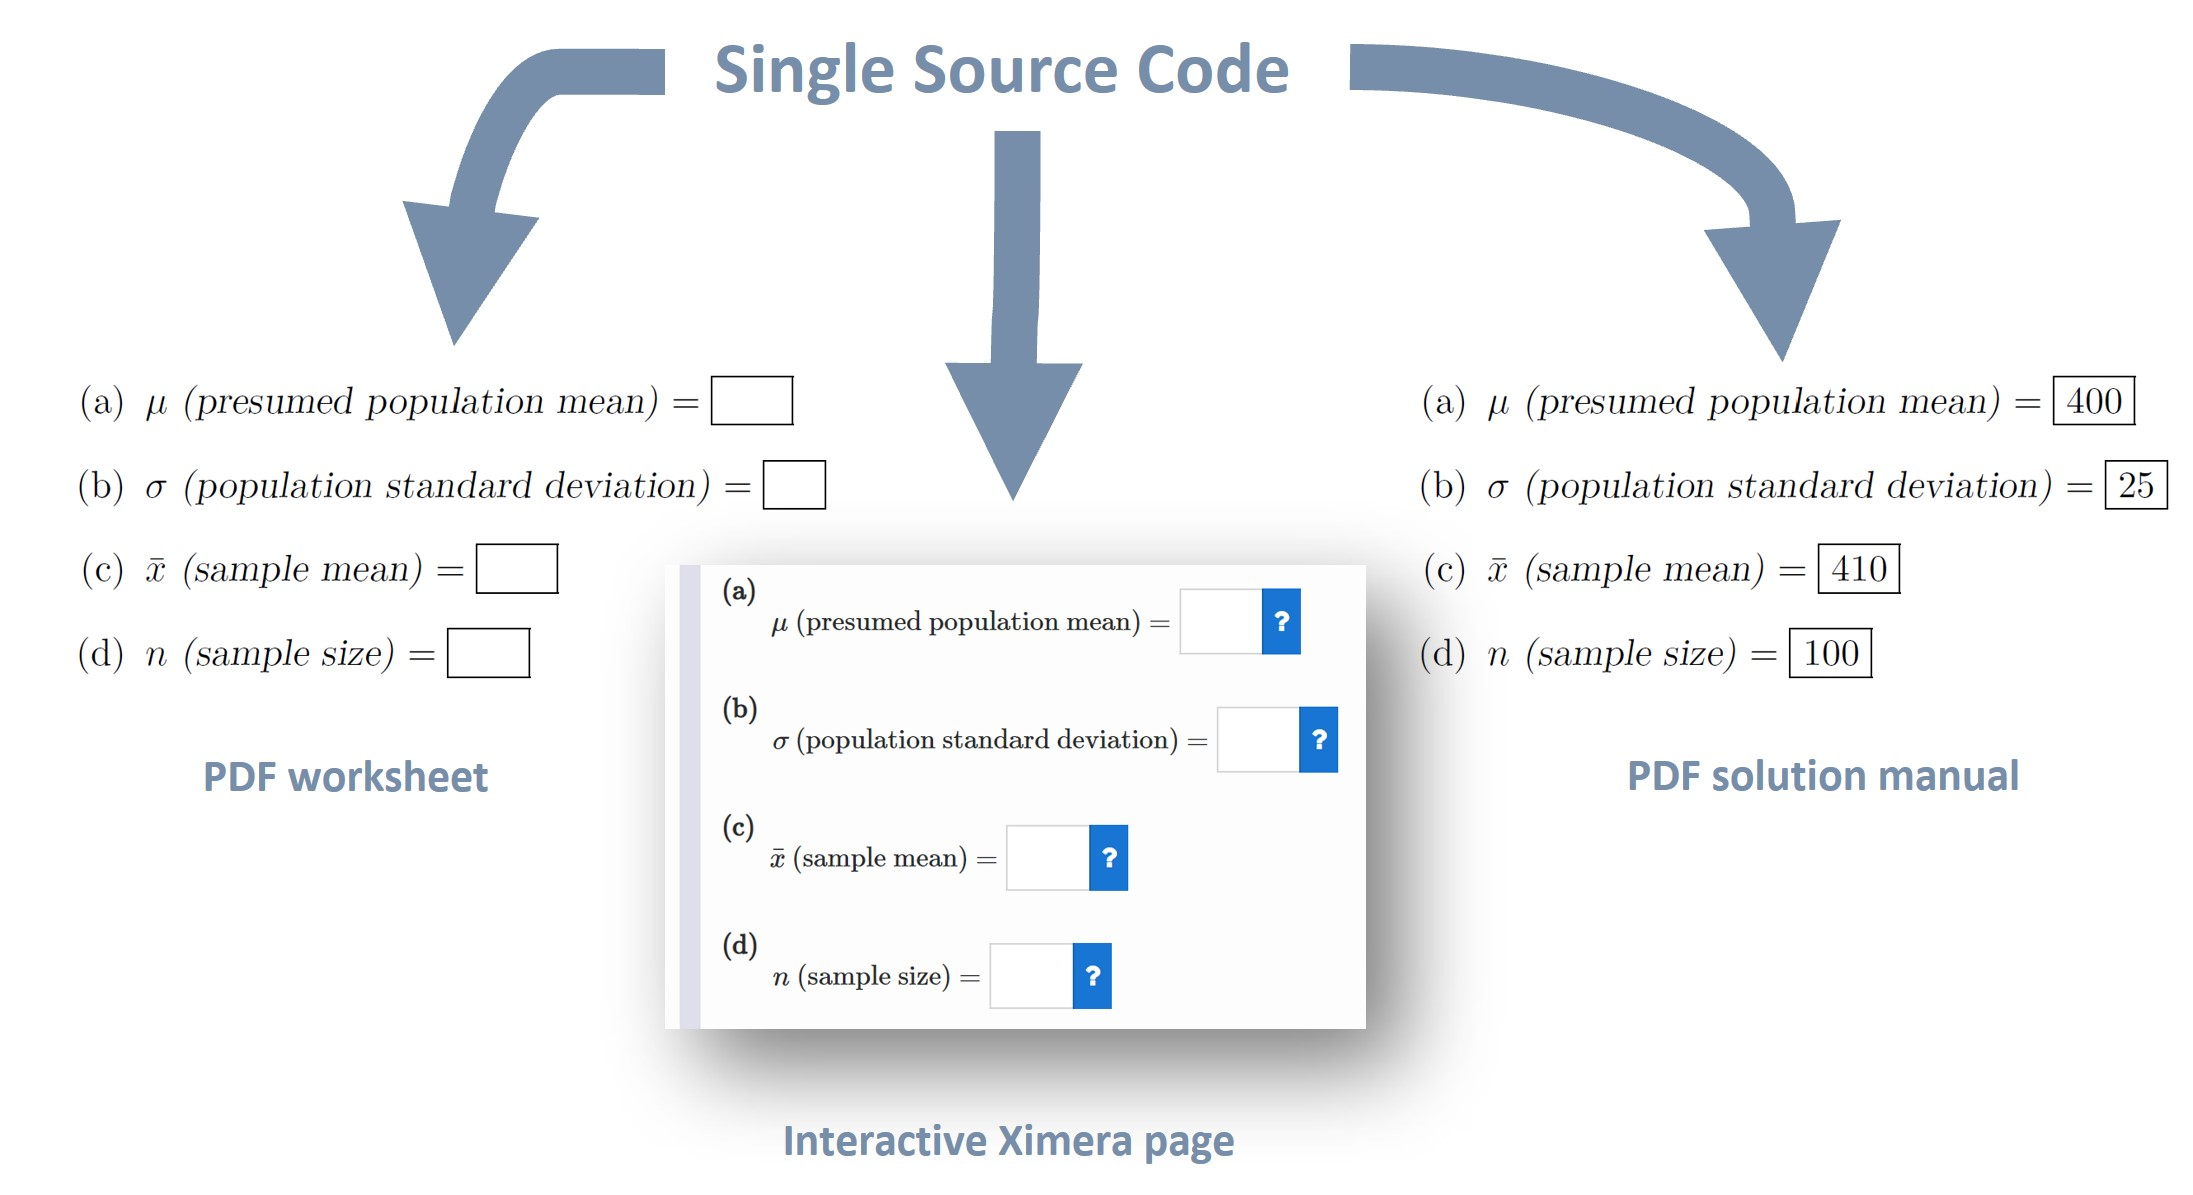
\includegraphics{SimultaneousOutput.jpg}
  }
\end{center}
\end{frame}

\begin{frame}{Ximera history}
  \begin{itemize}[<+->]
    \item 2010: \LaTeX\ to (interactive) app on iPad, by Bart Snapp et al.
    \item 2012/2013: MOOCulus and Calculus One, by Jim Fowler et al.
    \item 2013-2016: Grant DUE-1245433  'Interactive Textbook' \\  Jim Fowler, Bart Snapp et al.
    \item 2016-: many courses are developed, and published on \url{https://ximera.osu.edu}
    \item 2016: Ximera-server at University of Florida \\ Jason Nowell; variant Xronos with extra functionality
    \item 2019: Ximera-server at KU Leuven, Belgium \\ Jesse Hoobergs and Wim Obbels; docker, layout, extra functionality
    \item 2024-2026: grant from 'Open Textbooks Pilot Program'
  \end{itemize}

\end{frame}

\begin{frame}[t]{Example (HTML, OSU layout)}
  \begin{center}
    \resizebox{\linewidth}{!}{
      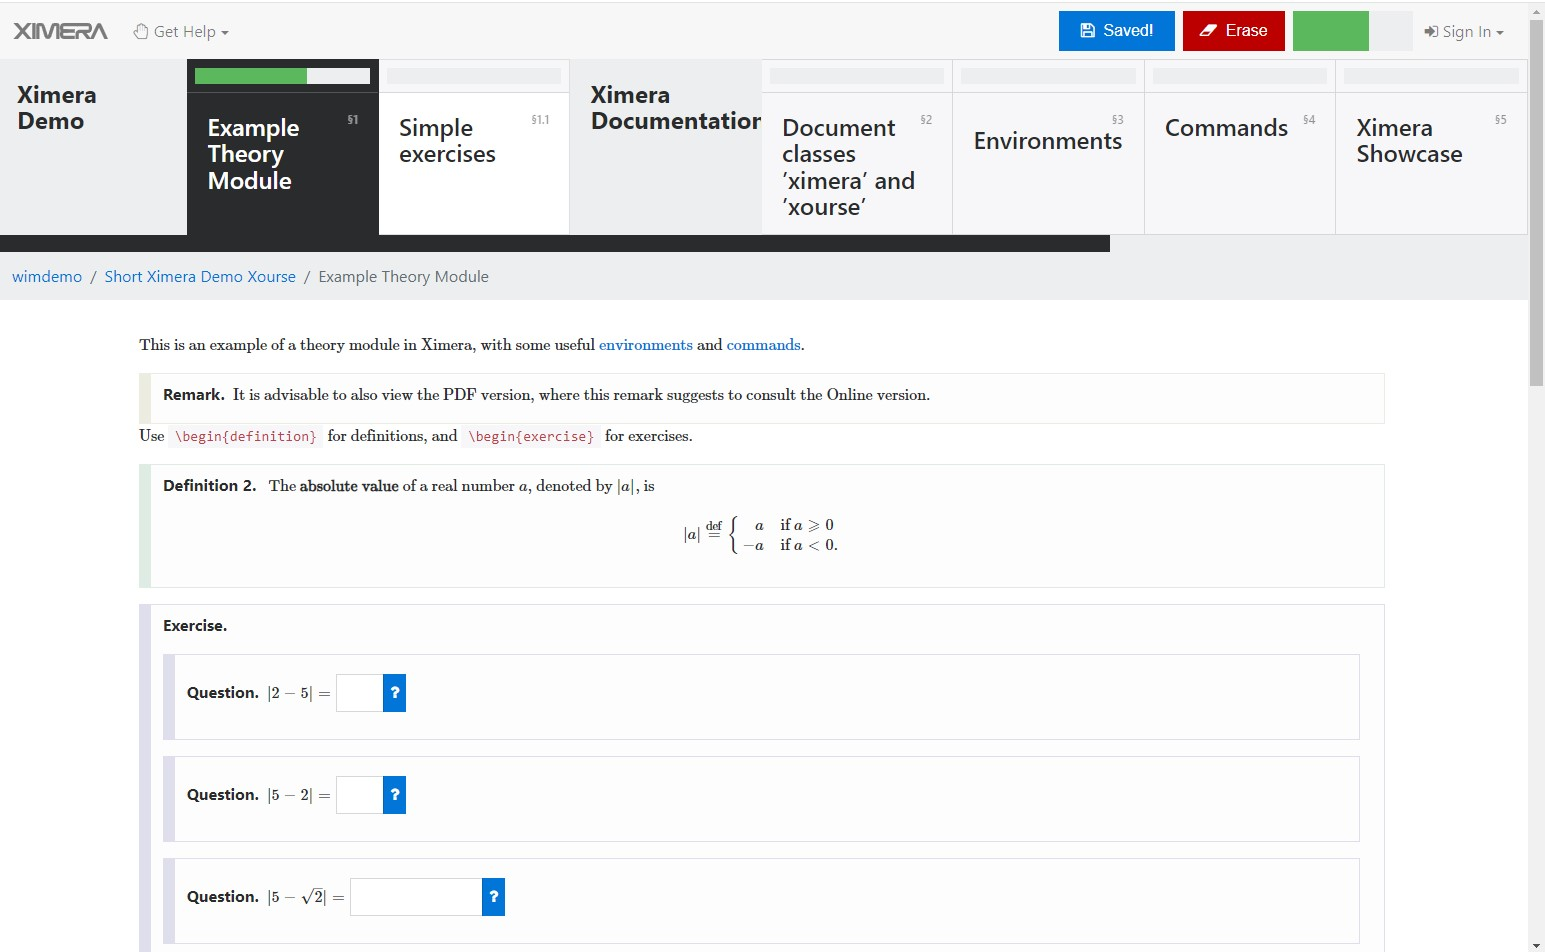
\includegraphics{demo_osu.jpg}
    }  
  \end{center}
\end{frame}

\begin{frame}[t]{Example (HTML, KU Leuven layout)}
  \begin{center}
    \resizebox{0.49\linewidth}{!}{
      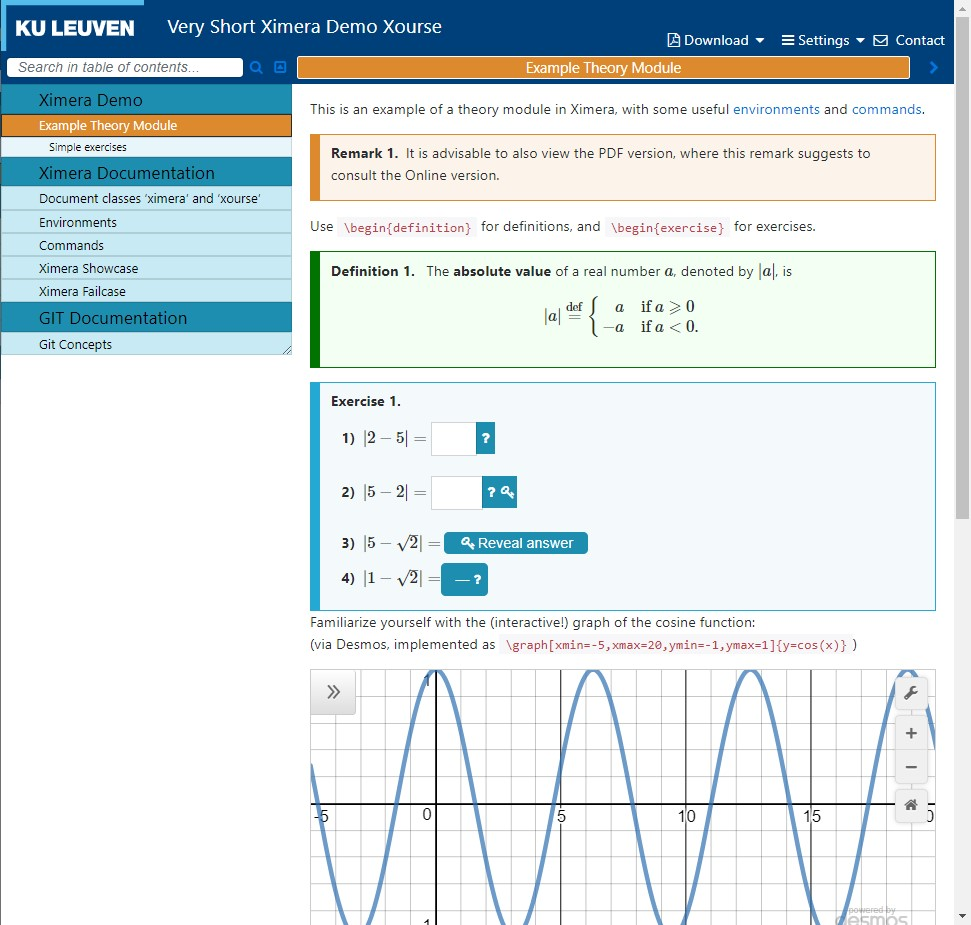
\includegraphics{demo_html.jpg}
    }  
    \resizebox{0.49\linewidth}{!}{
      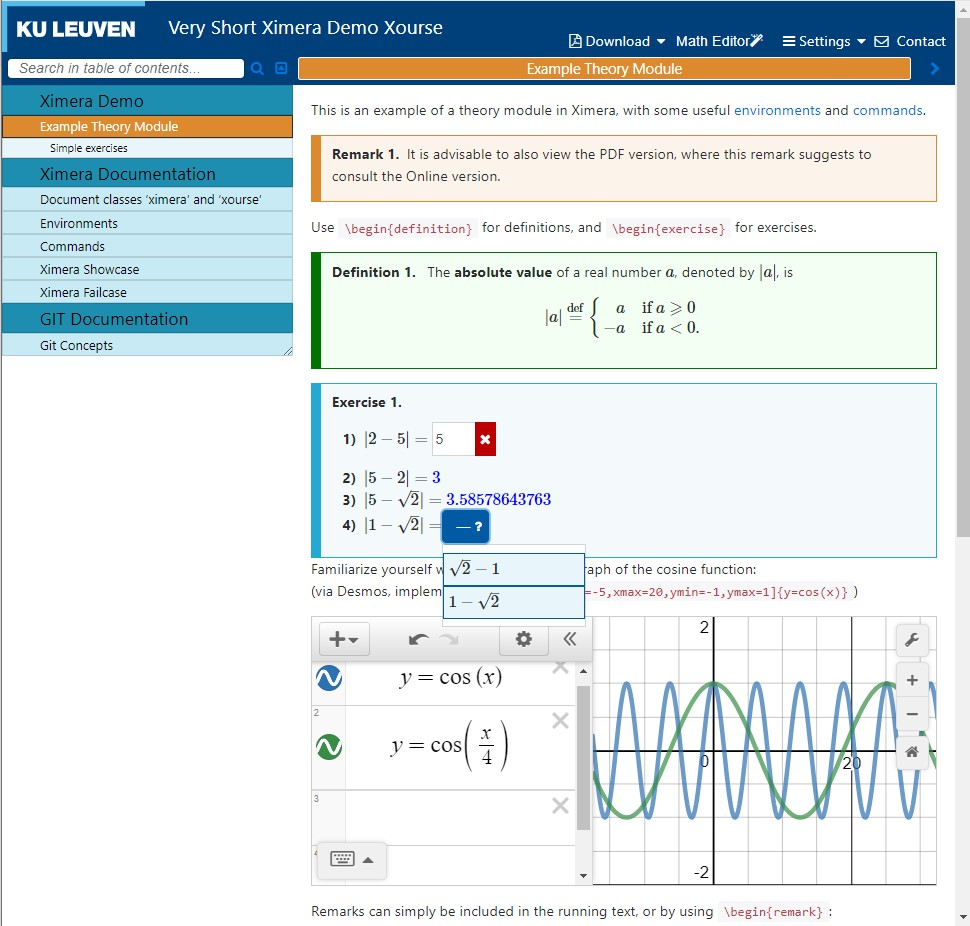
\includegraphics{demo_htmlanswers.jpg}
    }   
  \end{center}
\end{frame}

% \begin{frame}[t]{Example (HTML answered)}
%   \begin{center}
%     \resizebox{0.5\textwidth}{!}{
%       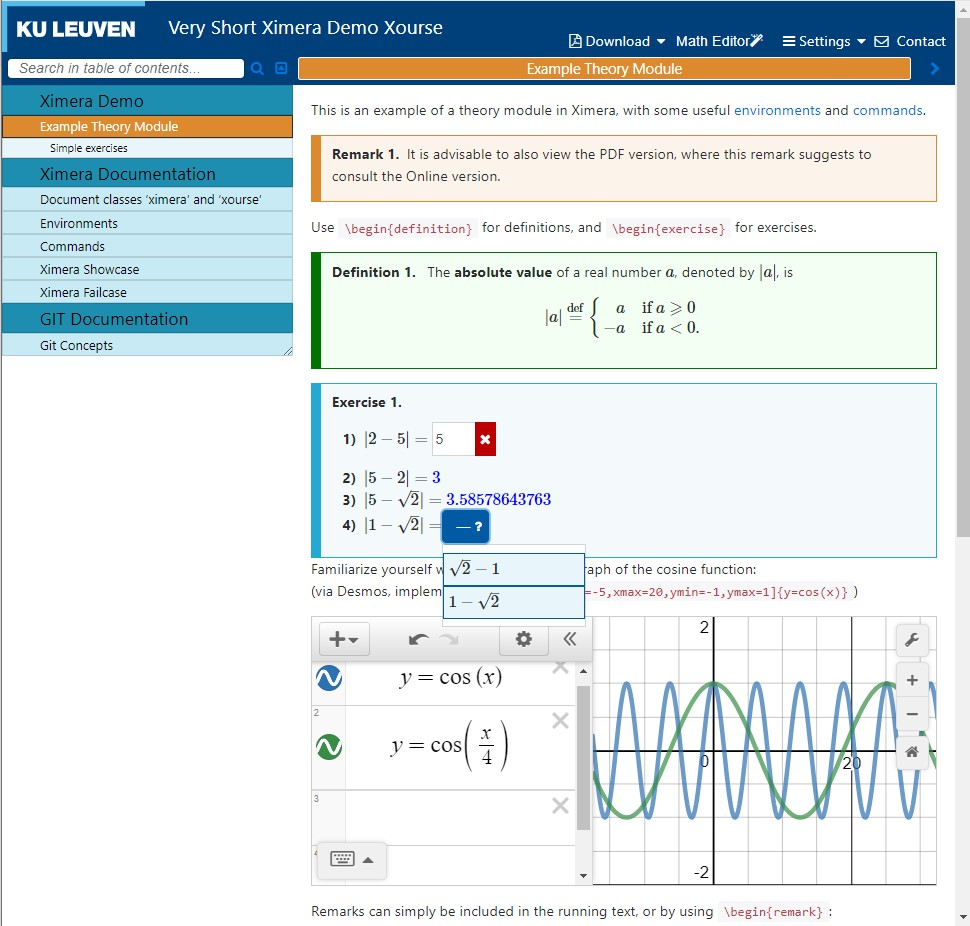
\includegraphics{demo_htmlanswers.jpg}
%     }  
%   \end{center}
% \end{frame}

\begin{frame}{Example (PDF activity)}
  \begin{center}
    \resizebox{0.49\linewidth}{!}{
      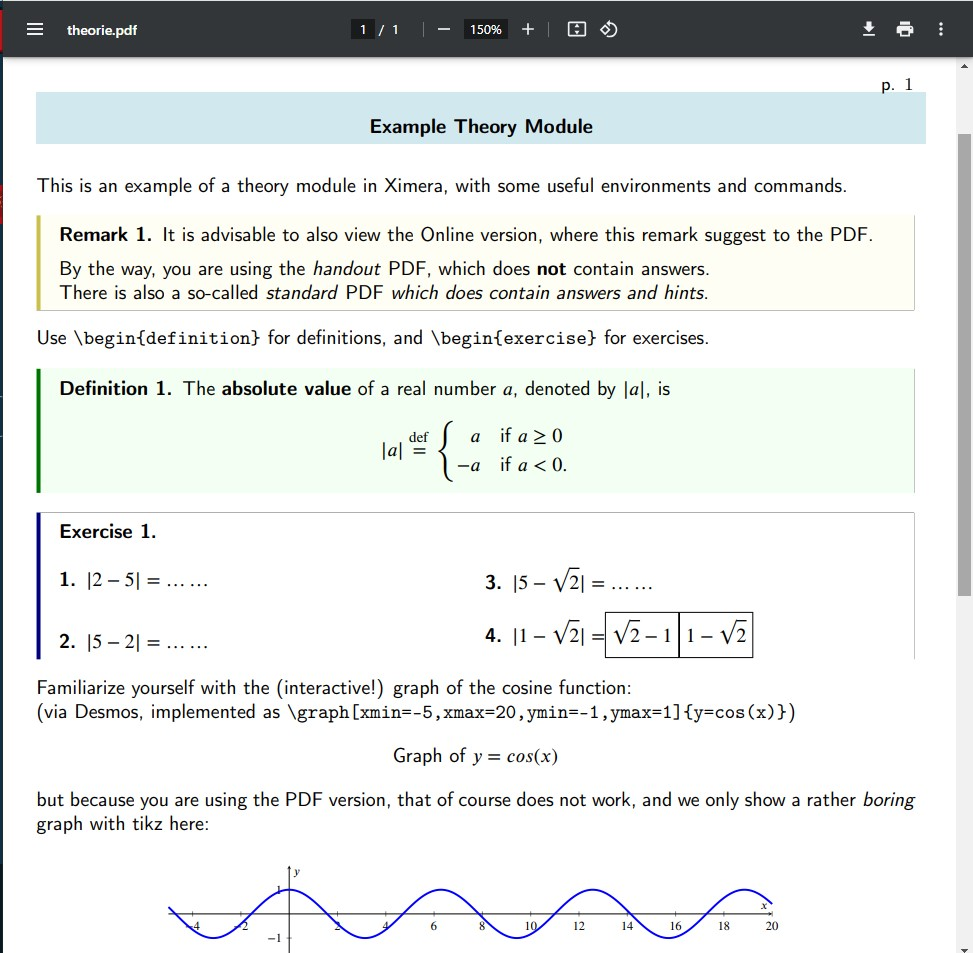
\includegraphics{demo_handout.jpg}
    }  
    \resizebox{0.49\linewidth}{!}{
      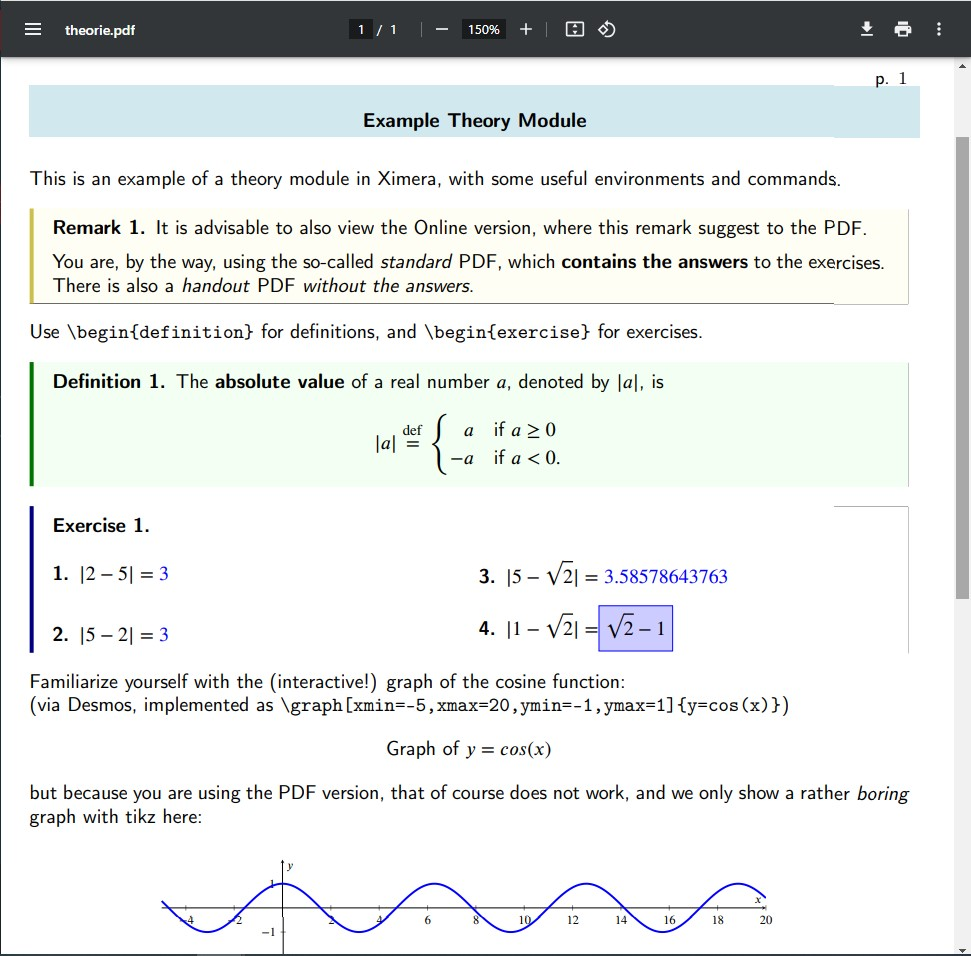
\includegraphics{demo_standard.jpg}
    }    
  \end{center}
\end{frame}

% \begin{frame}{Example (with answers)}
%   \begin{center}
%     \resizebox{0.5\textwidth}{!}{
%       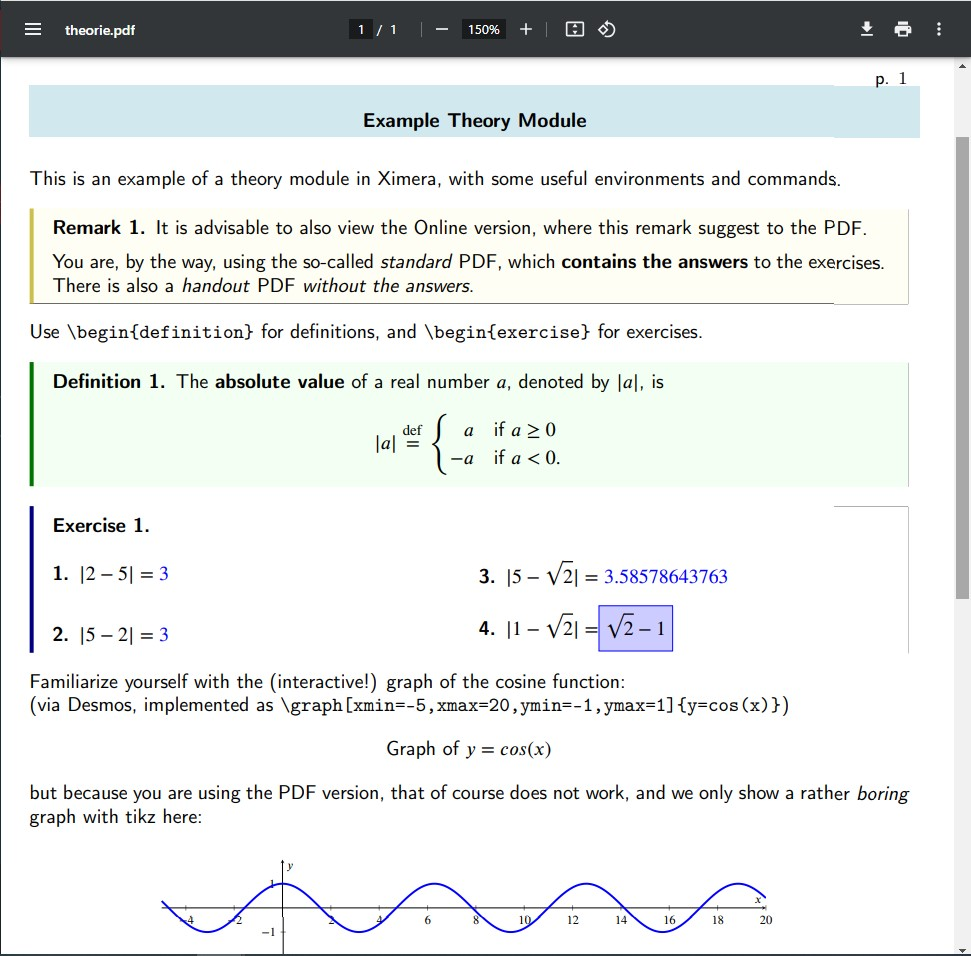
\includegraphics{demo_standard.jpg}
%     }  
%   \end{center}
% \end{frame}

\begin{frame}{Example (PDF xourse)}
  \begin{center}
    \resizebox{0.49\linewidth}{!}{
      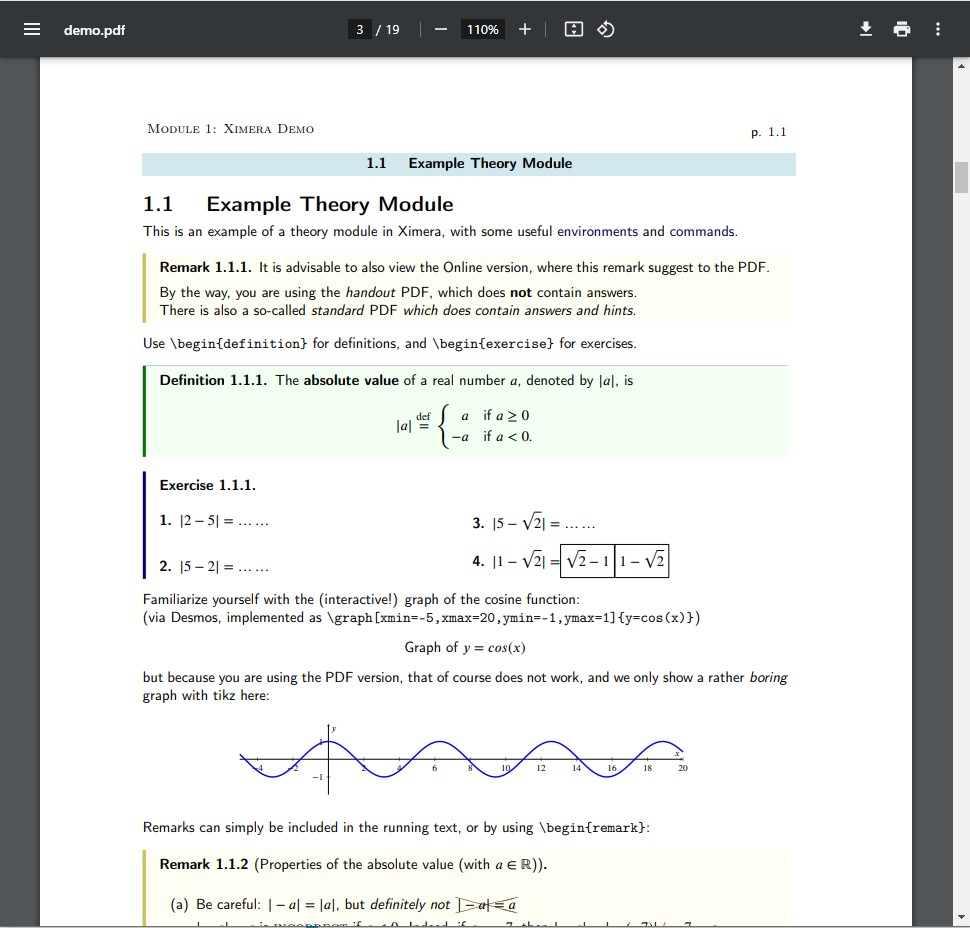
\includegraphics{demo_xourse.jpg}
    }     
    \resizebox{0.49\linewidth}{!}{
      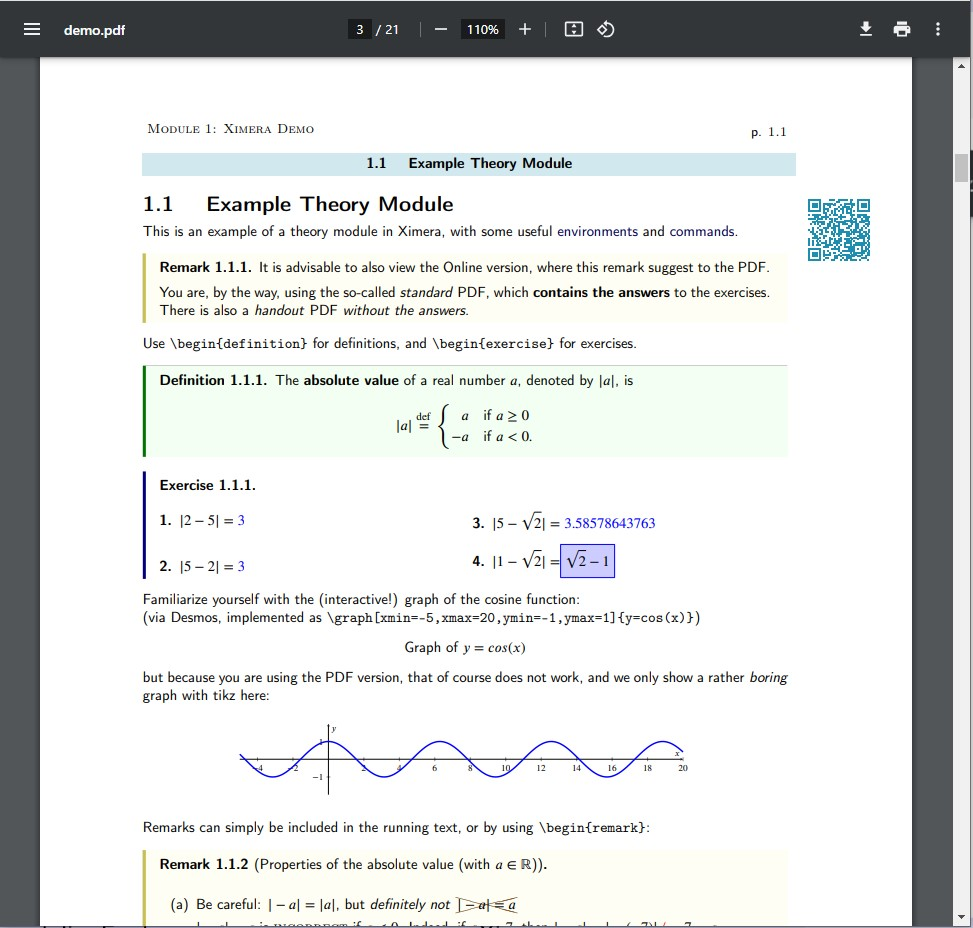
\includegraphics{demo_xourseanswers.jpg}
    }     
  \end{center}  
\end{frame}

% \begin{frame}{Example (in xourse)}
%   \begin{center}
%     \resizebox{0.7\textwidth}{!}{
%       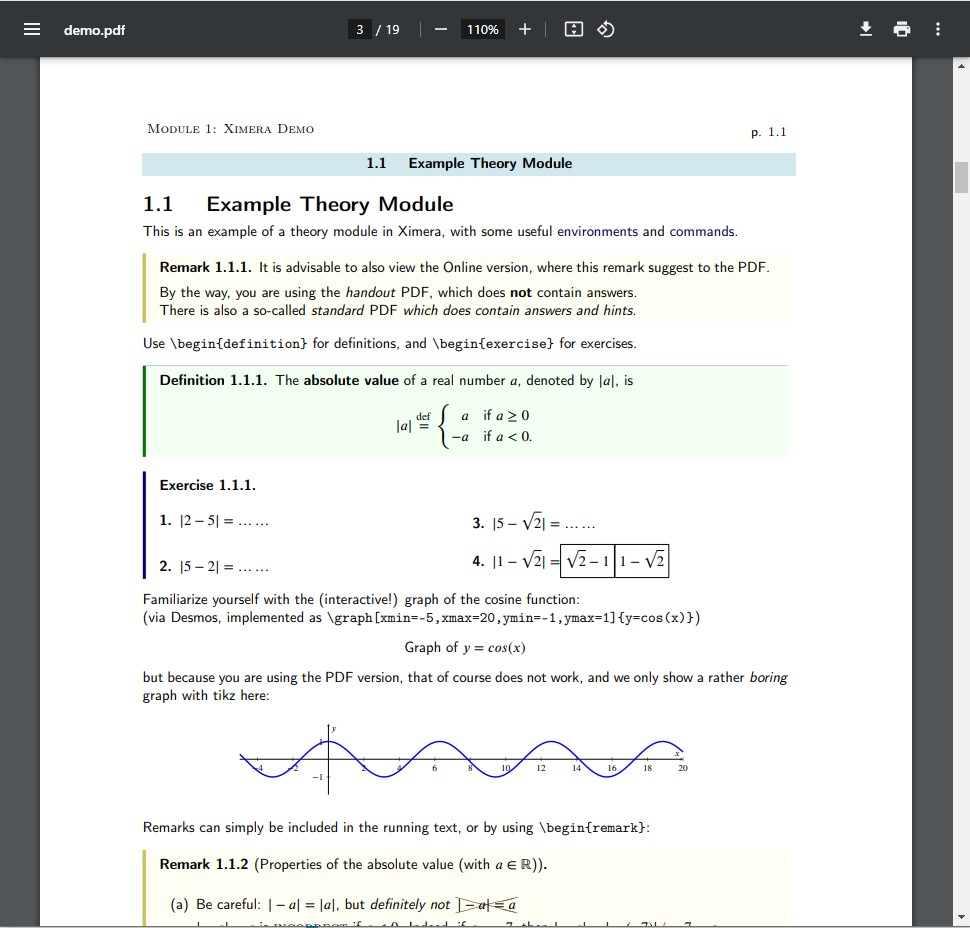
\includegraphics{demo_xourse.jpg}
%     }  
%   \end{center}
% \end{frame}


\begin{frame}{Example (source of activity (1))}
  \vspace{-0.3cm}
  \begin{center}
    \resizebox{0.75\textwidth}{!}{
      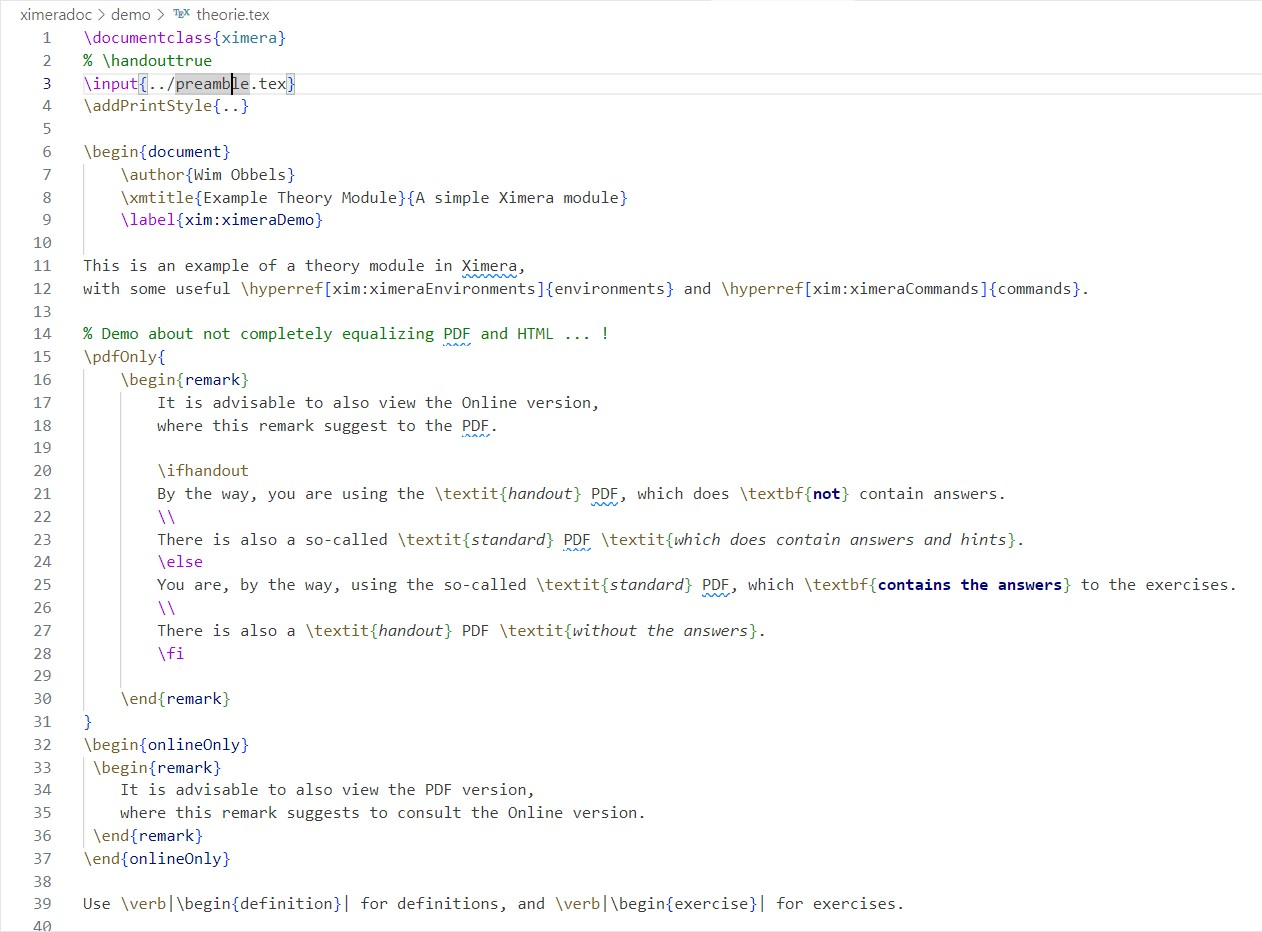
\includegraphics{demo_source1.jpg}
    }  
  \end{center}
\end{frame}

\begin{frame}{Example (source of activity (2))}
  \vspace{-0.3cm}  
  \begin{center}
    \resizebox{0.75\textwidth}{!}{
      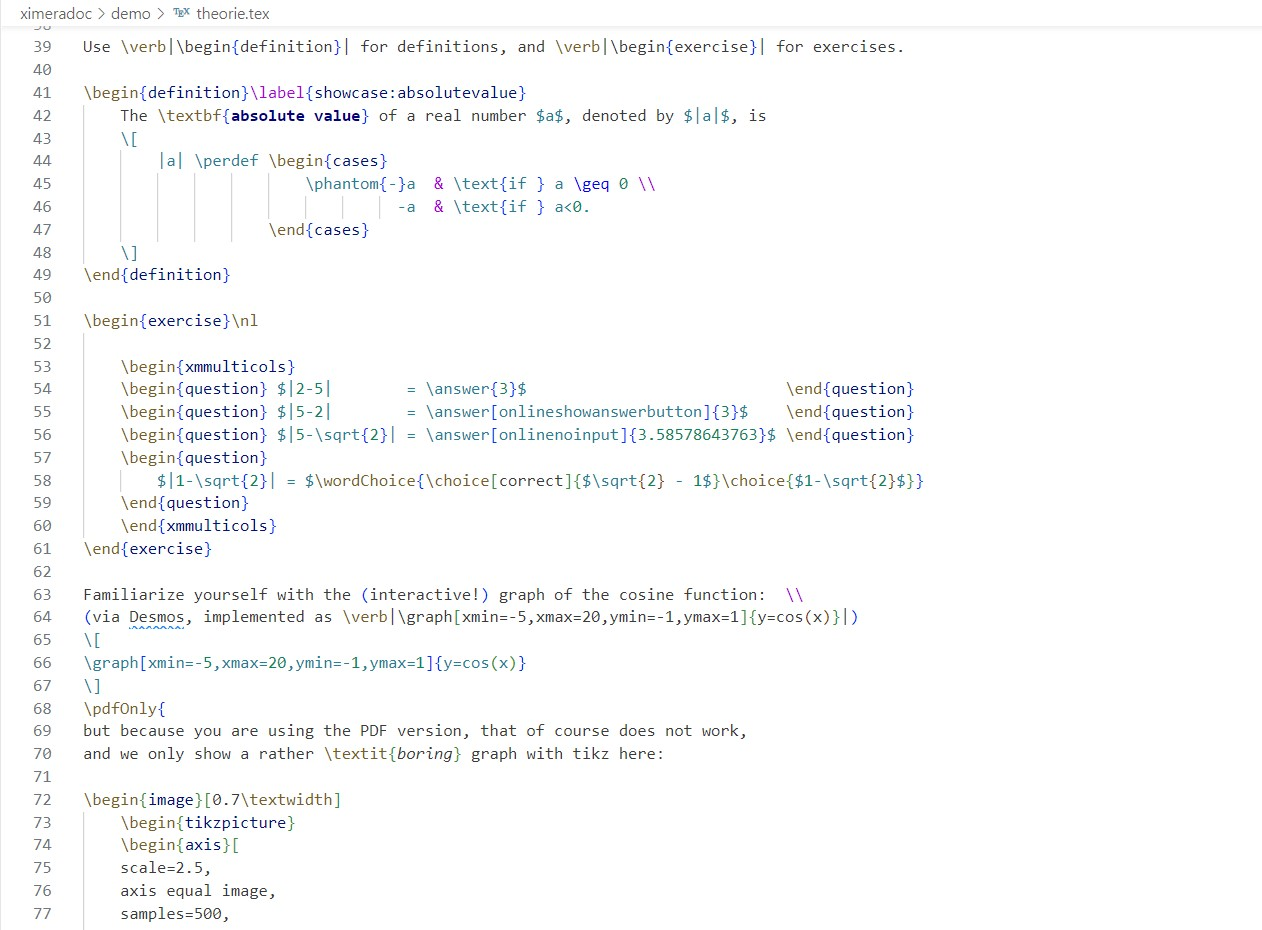
\includegraphics{demo_source2.jpg}
    }  
  \end{center}
\end{frame}

\begin{frame}{Example (source of xourse)}
  \vspace{-0.3cm}
  \begin{center}
    \resizebox{0.75\textwidth}{!}{
      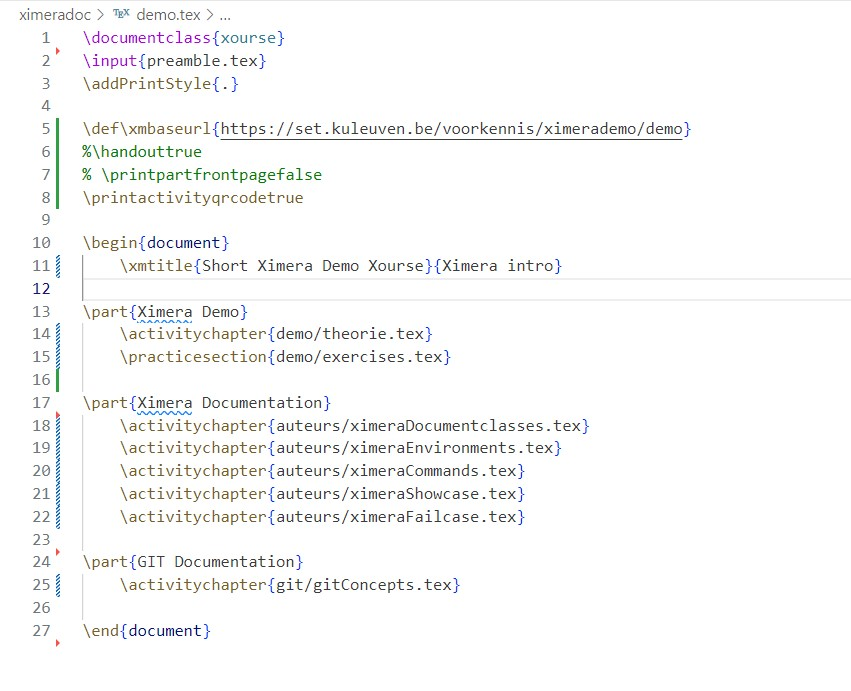
\includegraphics{demo_sourcexourse.jpg}
    }  
  \end{center}
\end{frame}


\begin{frame}[t]{Styling (HTML/HTML(alt)/PDF)}
  \begin{center}
    \resizebox{\textwidth}{!}{
      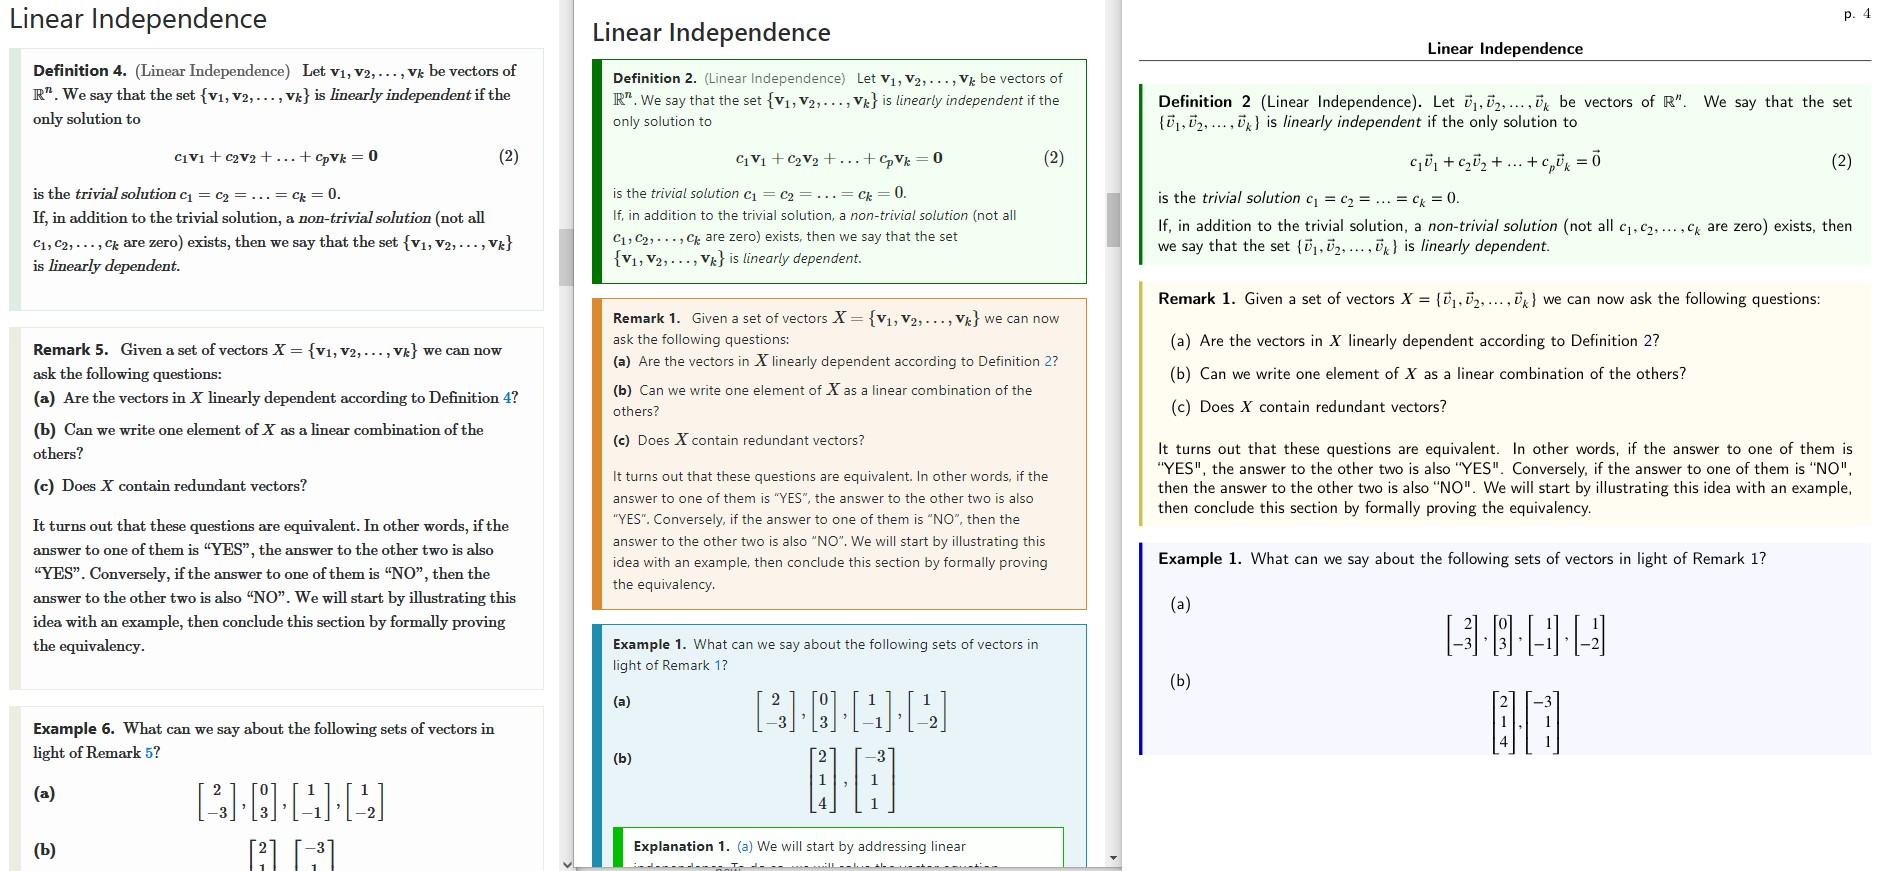
\includegraphics{Styling_LinearIndependence.jpg}
    }  
  \end{center}
\end{frame}

\begin{frame}{More Ximera features}
  \begin{itemize}
  \item hints/feedback/solutions; foldable environments
  \item answers with 'expressions' i.e. \texttt{$\rm{x}^2$-4} \quad vs \quad \texttt{-4+$\rm{x}^2$} \quad vs \quad \texttt{ (x  +  2)(x-2)}
  \item Integration of geogebra/youtube/google docs/xkcd
  \item LTI link to LMS (Blackboard/Moodle/\ldots); only LTI 1.1
  \item Integration of SAGE
  \item Downloadable student activity statistics
  \item Extra validators for answers (in javascript)
  \item \ldots
  \end{itemize}
\end{frame}

\begin{frame}[t]{Build Architecture ('classic')}

\begin{center}
\resizebox{0.9\linewidth}{!}{
\begin{tikzpicture}  

\node[block, fill=green,text width=6cm] (pcenduser) {
          Student
          \nodepart{three}
          - browser
};  

\node[block,right=3cm of pcenduser, fill= green,text width=10cm] (ximeraserver) {
          Ximera Server (public website)
          \nodepart{three} 
          \url{https://ximera.osu.edu}\\
          \url{https://set.kuleuven.be/voorkennis}
};          

\node[block, fill=orange!50!white,below=0.3cm of pcenduser, text width=6cm ] (pcauthor) {
    Author (classic)
    \nodepart{two}
    - \LaTeX\ installation \\
    - git client \\ 
    - editor \\
    - {\color{red}GPG key} \\
    - {\color{red}xake} \\
    - browser
    \nodepart{three} Procedure:\\
    - git clone course.git \\
    - edit \LaTeX\ code \\
    - git commit \\
    - xake bake/frost/serve
};  

\draw[line,->] (pcenduser.355) -- node[above] {} (ximeraserver.175);  
          
\draw[line,->] (pcauthor.320) -- node[right] {xake (https PUT)} (ximeraserver.175);  

\node[draw, fill=gray, fill opacity=0.1,inner xsep=5mm,inner ysep=6mm,
      fit=(ximeraserver),
      label={90:Cloud}] (icts) {};   


\end{tikzpicture}
  }
\end{center}

\end{frame}

\begin{frame}[t]{Build Architecture ('local docker')}

  \begin{center}
    \resizebox{0.9\linewidth}{!}{
    \begin{tikzpicture}  
    
    \node[block, fill=green,text width=6cm] (pcenduser) {
              Student
              \nodepart{three}
              - browser
    };  
    
    \node[block,right=3cm of pcenduser, fill= green,text width=10cm] (ximeraserver) {
              Ximera Server (public website)
              \nodepart{three} 
              \url{https://ximera.osu.edu}\\
              \url{https://set.kuleuven.be/voorkennis}
    };           

\node[block, fill=orange!50!white,below=0.3cm of pcenduser, text width=6cm ] (pcauthor) {
    Author (local docker)
    \nodepart{two}
    - \textbf{docker} (contains xake/TeXLive)\\
    - git client\\ 
    - editor (strong suggestion: VSCode) \\
    - {\color{red}GPG key} \\
    \phantom{- xake}\\
    - browser
    \nodepart{three} Procedure:\\
    - git clone course.git \\
    - edit \LaTeX code \\
    - git commit \\
    - \textbf{docker} xake bake/frost/serve
};  

\draw[line,->] (pcenduser.355) -- node[above] {} (ximeraserver.175);  
          
\draw[line,->] (pcauthor.320) -- node[right] {xake (https PUT)} (ximeraserver.175);  

\node[draw, fill=gray, fill opacity=0.1,inner xsep=5mm,inner ysep=6mm,
      fit=(ximeraserver),
      label={90:Cloud}] (icts) {};   


\end{tikzpicture}
  }
\end{center}

\end{frame}


\begin{frame}[t]{Build Architecture ('cloud')}

  \begin{center}
    \resizebox{0.9\linewidth}{!}{
    \begin{tikzpicture}  
    
    \node[block, fill=green,text width=6cm] (pcenduser) {
              Student
              \nodepart{three}
              - browser
    };  
    
    \node[block,right=3cm of pcenduser, fill= green,text width=10cm] (ximeraserver) {
              Ximera Server (public website)
              \nodepart{three} 
              \url{https://ximera.osu.edu}\\
              \url{https://set.kuleuven.be/voorkennis}
    };          

\node[block, fill=orange!50!white,below=0.3cm of pcenduser, text width=6cm ] (pcauthor) {
    Author (local/cloud docker)
    \nodepart{two}
    - docker \\
    - git client\\ 
    - editor (strong suggestion: VSCode) \\
    \phantom{- GPG key}\\ 
    \phantom{- xake}\\
    - browser
    \nodepart{three} Procedure:\\
    - git clone course.git \\
    - edit \LaTeX code \\
    - git commit \\
    - (optional) docker xake bake \\
    - \textbf{git push}
};  

\node[block, fill=orange!50!white,below =of ximeraserver,text width=10cm     ] (gitrepo) {
  Github/GITLAB Repository Server
  \nodepart{two}
    - repo xourse.git \\
    - docker image repository \\
    - GPG Key(s) \\
    - Authentication and Authorization
    \nodepart{two}
    Actions or Pipelines for \\
    - docker xake bakePdf  (with and/or without answers) \\
    - docker xake bake/frost/serve
    \nodepart{three}
       \url{https://gitlab.kuleuven.be} \\
       \url{https://github.com}
    };  

    \node[draw, fill=gray, fill opacity=0.1,inner xsep=5mm,inner ysep=6mm,
      fit=(ximeraserver)(gitrepo),
      label={90:Cloud}] (icts) {};   


\draw[line,->] (pcenduser.355) -- node[above] {} (ximeraserver.175);  
          
% \draw[line,->] (pcauthor.320) -- node[right] {xake (https PUT)} (ximeraserver.175); 

\draw[line,->] (pcauthor.315) -- node[pos=0.2,below right] {push/pull} (gitrepo.170);  

\draw[line,->] (gitrepo) -- node[right] {xake} (ximeraserver);  

\end{tikzpicture}
  }
\end{center}
\end{frame}

\begin{frame}{Further developments}

  \begin{itemize}[<+->]
  \item Accessibility  (both HTML and PDF)
  \item Grade and performance database and dashboard
  \item LTI 1.3 support
  \item TeX-in-the-browser \\ \url{https://people.math.osu.edu/fowler.291/latex/}
  \item Better documentation
  \item Better VSCode/docker/cloud support
  \end{itemize}

\end{frame}

\begin{frame}{Grants}

  Grants from \$500 to \$5000 are available for concrete contributions.
  
  Contact: ximera@math.osu.edu

\end{frame}

\begin{frame}[t]{\centering Thanks for listening.}

  
  \vfill
  \textbf{\Large Questions:} ask them right now, or mail them.
  \vfill
  \begin{itemize}
  \item \url{https://github.com/XimeraProject}
  \item \url{https://ximera.osu.edu/testing/examples}
  \item \url{https://set.kuleuven.be/voorkennis/examples/examples}
  \item \url{https://people.math.osu.edu/fowler.291/latex/}
  % \item (discord/zulip/... .?)
  \end{itemize}
  \vfill

  Contact: \\[0.5cm]

  \begin{tabular}{ll}
    About Ximera, grants etc.: & ximera@math.osu.edu    (Bart Snapp, Jim Fowler) \\
    About this talk :          & wim.obbels@kuleuven.be
  \end{tabular}    
  \vfill
\end{frame}


\end{document}